\documentclass{beamer}
%
% Choose how your presentation looks.
%
% For more themes, color themes and font themes, see:
% http://deic.uab.es/~iblanes/beamer_gallery/index_by_theme.html
%
\mode<presentation>
{
  \usetheme{default}      % or try Darmstadt, Madrid, Warsaw, ...
  \usecolortheme{default} % or try albatross, beaver, crane, ...
  \usefonttheme{default}  % or try serif, structurebold, ...
  \setbeamertemplate{navigation symbols}{}
  \setbeamertemplate{caption}[numbered]
} 

\usepackage[english]{babel}
\usepackage[utf8x]{inputenc}

\usepackage{tabularx}
\usepackage{multirow}
\usepackage{booktabs}
\usepackage{tikz}

\title[]{Version Control Tool: Git}
\author{Biao Wang}
\institute{Anacode}
\date{\today}

\begin{document}

\begin{frame}
  \titlepage
\end{frame}

% Uncomment these lines for an automatically generated outline.
% \begin{frame}{Outline}
%  \tableofcontents
% \end{frame}

\section{Introduction}
\begin{frame}{Introduction}
    \begin{itemize}
      \item make your work organized      
    \end{itemize}  
    \begin{figure}
      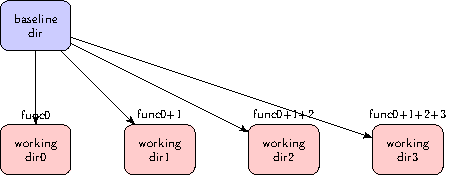
\includegraphics[width=.7\textwidth]{figures/withoutversioncontrol.pdf}      
    \end{figure}
    \begin{figure}
      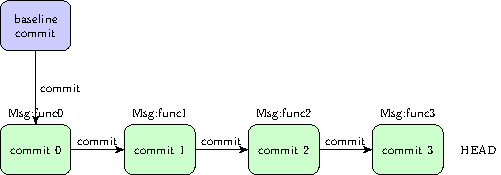
\includegraphics[width=.7\textwidth]{figures/withversioncontrol.pdf}
    \end{figure}         
\end{frame}

\begin{frame}{Introduction}
    \begin{itemize}
      \item debug your code
        \begin{itemize}
            \item make your life easy by narrowing down the problemetic code      
            \item But..., every commit shoud be verified before commit        
        \end{itemize}          
        \begin{figure}
        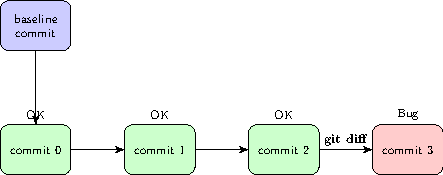
\includegraphics[width=.7\textwidth]{figures/debugversioncontrol.pdf}
        \end{figure}         
     \item teamwork development
        \begin{itemize}
            \item without version control tool, code management become extremely difficult.
        \end{itemize}          
    \end{itemize} 
\end{frame}

\section{Understanding git}
\begin{frame}{Understanding git: file status within git}
    \begin{figure}
    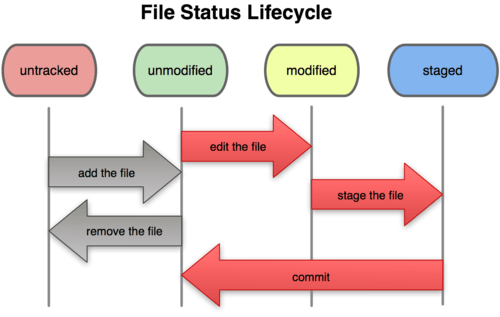
\includegraphics[width=.7\textwidth]{figures/gitlifestyle.png}
    \caption{\label{git life cycle} source: internet.}
    \end{figure}             
\end{frame}

\begin{frame}{Understanding git: file status within git}
    Demo: how file status changes
    \begin{itemize}
     \item    add file: \textbf{git add          }
     \item modify file: \textbf{                 }
     \item  stage file: \textbf{git add (-u)     }
     \item commit file: \textbf{git commit -m ``Msg for this commit''}
     \begin{itemize}
        \item bad commit message: ``fix some bugs''
        \item would be better: ``fix SIMD memory load bugs within deblockingfilter.cpp''
     \end{itemize}
     \item remove file: \textbf{git remove       }
    \end{itemize}
\end{frame}

\begin{frame}{How to use git}
\begin{itemize}
\item Use \texttt{tabular} for basic tables --- see Table~\ref{tab:widgets}, for example.
\item You can upload a figure (JPEG, PNG or PDF) using the files menu. 
\item To include it in your document, use the \texttt{includegraphics} command (see the comment below in the source code).
\end{itemize}

% Commands to include a figure:
%\begin{figure}
%\includegraphics[width=\textwidth]{your-figure's-file-name}
%\caption{\label{fig:your-figure}Caption goes here.}
%\end{figure}

\begin{table}
\centering
\begin{tabular}{l|r}
Item & Quantity \\\hline
Widgets & 42 \\
Gadgets & 13
\end{tabular}
\caption{\label{tab:widgets}An example table.}
\end{table}

\end{frame}

% \subsection{Mathematics}

\begin{frame}{Readable Mathematics}

% Let $X_1, X_2, \ldots, X_n$ be a sequence of independent and identically distributed random variables with $\text{E}[X_i] = \mu$ and $\text{Var}[X_i] = \sigma^2 < \infty$, and let
% $$S_n = \frac{X_1 + X_2 + \cdots + X_n}{n}
%       = \frac{1}{n}\sum_{i}^{n} X_i$$
% denote their mean. Then as $n$ approaches infinity, the random variables $\sqrt{n}(S_n - \mu)$ converge in distribution to a normal $\mathcal{N}(0, \sigma^2)$.

\end{frame}

\end{document}
